\section{Introduction and Motivation}

	\begin{frame}
		\frametitle{Latest Approaches}
	    \begin{columns}[T]
	        \begin{column}{0.49\textwidth}
	            \begin{itemize}%[<+->] Kommentar entfernen falls jeder Punkt einzeln erscheinen soll
					\item <1-4> \onslide<1->{Environment Previous Knowledge}\\[0.5cm]
					\item \onslide<3->{ROS Navigation Stack Setup}
	        	\end{itemize}
	        \end{column}
	        \begin{column}{0.49\textwidth}
	        	\begin{itemize}%[<+->] Kommentar entfernen falls jeder Punkt einzeln erscheinen soll
	        		\item \onslide<2->{Global Planner}\\[0.3cm]
	        		\item \onslide<4>{Maximum speed $\leq 1.5 m/s$}
	        	\end{itemize}
	        \end{column}
	    \end{columns}
    	\centering
    	\onslide<3->{\includegraphics[scale=0.3]{pictures/navi_ros.png}}
	\end{frame}

	\begin{frame}
		\frametitle{Planner Requirements}
		\begin{columns}[T]
			\begin{column}{0.45\textwidth}
				\begin{itemize}%[<+->] Kommentar entfernen falls jeder Punkt einzeln erscheinen soll
					\item Robot localization using: 
					\begin{itemize}
						\item Laser Scanner
						\item Map
						\item Robot's current estimated location
					\end{itemize}
				\end{itemize}
			\end{column}
			\begin{column}{0.49\textwidth}
				\includegraphics[scale=0.7]{pictures/navigation_ros_2.pdf}
			\end{column}
		\end{columns}
	\end{frame}

	\begin{frame}
		\frametitle{Motivation}
		\begin{block}{Proposed Approach}
			\begin{itemize}
				\pause
				\item On-line trajectory planning
				\pause
				\item Does not require \textit{global planner}
				\pause
				\item Does not demand \textit{map}
				\pause
				\item Can operate in environment accommodating dynamic obstacles, e.g. \textit{(pedestrian, multi-robots)}  
				\pause
				\item Robot speed $> 1.5 m/s$
			\end{itemize}
		\end{block}
	\end{frame}

	\begin{frame}
		\frametitle{Proposed Approach}
		\begin{columns}[T]
			\begin{column}{0.45\textwidth}
				\begin{itemize}%[<+->] Kommentar entfernen falls jeder Punkt einzeln erscheinen soll
					\item Robot localization \\[0.5cm]
					\item Obstacles location
				\end{itemize}
			\end{column}
			\begin{column}{0.49\textwidth}
				\includegraphics[scale=0.8]{pictures/navigation_ros_3.pdf}
			\end{column}
		\end{columns}
	\end{frame}

	\begin{frame}
		\frametitle{Model Predictive Control}
		\centering
		\only<1>{\animategraphics[loop,controls,width=0.7\linewidth]{2}{pictures/mpc_group/MPC_scheme_basic-}{0}{6}}
		\only<2>{\includegraphics[scale=1.0]{pictures/mpc_group/MPC_scheme_basic-7.pdf}}
	\end{frame}

	\begin{frame}
		\frametitle{NMPC Optimization Problem Schematic}
		\centering
		\only<1>{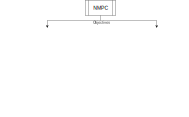
\includegraphics[scale=0.7]{pictures/mpc_planner_group/mpc_planner_0.pdf}}
		\only<2>{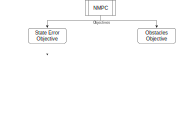
\includegraphics[scale=0.7]{pictures/mpc_planner_group/mpc_planner_1.pdf}}
		\only<3>{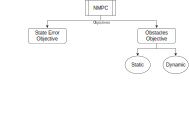
\includegraphics[scale=0.7]{pictures/mpc_planner_group/mpc_planner_2.pdf}}
		\only<4>{\includegraphics[scale=0.7]{pictures/mpc_planner_group/mpc_planner_3.pdf}}
		\only<5>{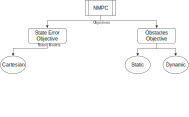
\includegraphics[scale=0.7]{pictures/mpc_planner_group/mpc_planner_4.pdf}}
		\only<6>{\includegraphics[scale=0.7]{pictures/mpc_planner_group/mpc_planner_5.pdf}}
		\only<7>{\includegraphics[scale=0.7]{pictures/mpc_planner_group/mpc_planner_6.pdf}}
	\end{frame}



	\begin{frame}
		\frametitle{Was sind Daten?}
		\pause
		Je nach Fachbereich werden verschiedene, teilweise sehr ähnliche, Definitionen verwendet. Hier orientieren wir uns an folgender Definition:
		\pause
		\begin{block}{Daten}
		''reinterpretable representation of information in a formalized manner suitable for communication, interpretation, or processing''\footnote{ISO/IEC 2382:2015}
		\end{block}
		\pause
		\begin{itemize}
		\item Daten sind hier also eine (digitale) formalisierte Darstellung von Informationen
		\pause
		\item Die Informationen sind wieder interpretierbar
		\pause
		\item Die formalisierte Darstellung ist so geschaffen, dass die Informationen für Kommunikation, Interpretation und Auswertung verwendet werden können 
		\end{itemize}
	\end{frame}



\begin{frame}
\frametitle{Anwendungen für (komplexe) Datenanalysen}
\begin{itemize}[<+->]
\item Sortierung von Briefen mittels automatisierter Erkennung von handschriftlichen Adressen
\item Erkennung von Gegenständen für automatisiertes Picking
\item Predictive Maintenance
\item Routenplanung
\item Autonome Roboter und Fahrzeuge
\item Analyse von Kundenverhalten
\item Prognose von Durchlaufzeiten, Mitarbeiterbedarf,...
\item Anomalieerkennung in der Fertigung
\end{itemize}
\end{frame}